\chapter{Konzeption}\label{chap:concept}
(Idea Generation erste Iteration)

Bei der Konzeption der eigenen Android-App liegt der Fokus auf der Erfüllung aller in Kapitel 4 als relevant klassifizierten Kriterien.
Hierzu werden im Folgenden Ideen vorgestellt, die in einem ersten Prototyp umgesetzt werden sollen.

\section{Sichtbarkeit des Systemzustandes}

\begin{wrapfigure}{R}{0.5\textwidth}
  \centering
  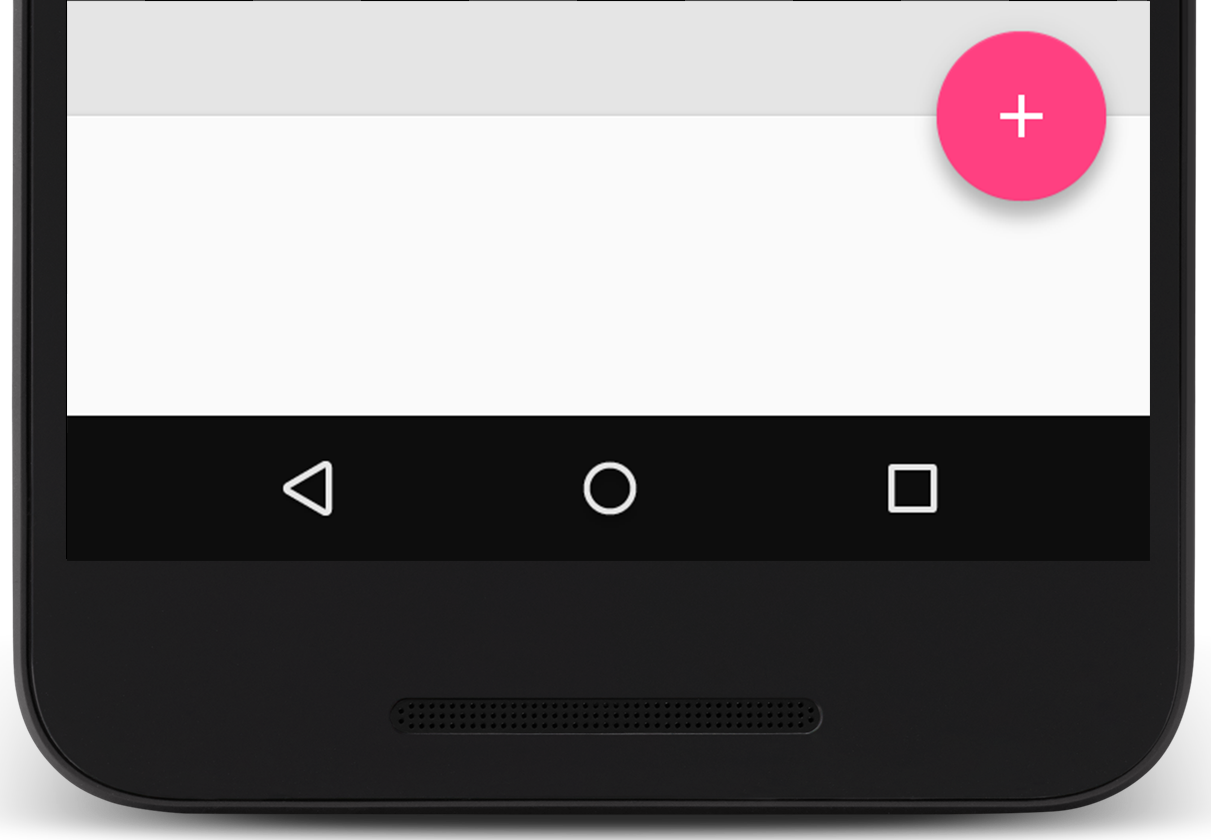
\includegraphics[keepaspectratio, width=0.5\textwidth]{fab}
  \caption{Floating Action Button}
  \label{fig:fab}
\end{wrapfigure}

Um dem Benutzer zu jeder Zeit einen Überblick über den Systemzustand der App zu ermöglichen, soll ein \emph{Floating Action Button} (siehe \autoref{fig:fab}) eingesetzt werden, da dieser nicht viel Platz auf dem Bildschirm einnimmt, für den Benutzer dennoch jederzeit leicht zugänglich ist.
So schreibt \citeauthor{SJ16} in seiner Usability-Studie zum Vergleich eines traditionellen Buttons mit einem \emph{FAB}, dass die Nutzung eines \emph{Floating Action Buttons} dazu führe, dass Aufgaben, nachdem sie einmal mit dem \emph{FAB} erfolgreich ausgeführt wurden, anschließend effizienter durchgeführt werden können als mit einem traditionellen Button \citep[Seiten 14--16]{SJ16}.

\section{Übereinstimmung zwischen System und Welt}
Zusätzlich soll die App in einer natürlichen und logischen Reihenfolge benutzbar sein.
So soll dem Benutzer zuerst die Möglichkeit gegeben werden, ein gewünschtes Bild auszuwählen, welches im Anschluss daran in einer weiteren Benutzeroberfläche bearbeitet werden kann.
\todo{Hier workflow?}

\section{Benutzerkontrolle und -freieht}
Gerade die fehlende Undo/Redo-Funktionalität hat sich bei der App \pm{} in \autoref{subsec:pmeva} als  signifikantes Usability-Problem identifizieren lassen.
Aufgrund dessen soll diese Funktionalität über zwei dedizierte Icons in der Menüleiste angeboten werden, um potentielle Verwirrung wie in \autoref{subsec:imeva} bei der App \im{} zu vermeiden.
\todo{Menüleiste aus anderen Apps mit Redo/Undo}

\section{Konsistenz und Standards}
Um eine positive Benutzererfahrung zu generieren, und die Benutzung von nicht-intuitiven Icons zu vermeiden, werden bei der Implementierung die Design-Richtlinien von \emph{Google} befolgt.
Diese bieten sowohl Konzepte zur Umsetzung verschiedener Benutzeroberflächen-Elemente, als auch eine Vielzahl konsistent gestalteter Icons an.  \todo{ref auf Material-Guidelines}

\section{Fehlervorbeugung}
Zusätzlich soll das Deaktivieren von nicht-ausführbaren Aktionen dafür sorgen, dass Situationen, in denen Fehler entstehen können, präventiv vermieden werden.
Hierzu sollen nicht-benutzbare Icons ausgegraut und nicht auswählbar gestaltet werden.
\todo{disabled Icons in Apps}

\section{Wiedererkennung statt Erinnern}
Eine minimierte kognitive Belastung soll durch die Verwendung von gleichen Icons für gleiche Aktionen erzielt werden.
So soll im ``Zeichen-Modus'' als auch im ``Text-Modus'' ein Mülleimer-Icon in der Menüleiste die Möglichkeit bieten, die markierte Form bzw. den ausgewählten Text zu löschen.

\section{Flexibilität und Effizienz der Benutzung}
Der Benutzer soll in der Lage sein, die gezeichneten Formen im Nachhinein zu bearbeiten.
Hierzu soll es die Möglichkeit geben, dass der Benutzer bereits zu Beginn eine Standard-Farbe festlegen kann.
Diese soll dann für alle neu eingezeichneten Formen benutzt werden.
Zudem sollte es die Möglichkeit geben, einzelne Formen nachträglich anders färben zu können.
Abkürzungen für erfahrene Benutzer sollen durch das Einführen von verschiedenen Gesten gegeben werden.
So soll es zum Beispiel möglich sein, per Lang-Klick Geste auf eine Form Text eintragen zu können, anstatt erst in der Statusleiste den entsprechenden Button zu drücken.
Zudem soll die Möglichkeit bestehen, Texte im Nachhinein bearbeiten zu können, ohne diese erst löschen und dann neu erstellen zu müssen.
\todo{Lang-Klick Geste}

\section{Erkennbarkeit, Diagnose und Erholung von Fehlern}
Durch das präventive Vermeiden von Situationen, in denen Fehler auftreten können, sollte der Nutzer zu keiner Zeit in eine Fehlersituation gelangen können.
Sollte es dennoch zu einer solchen Situation kommen, so soll eine kurze, aber informative Nachricht in Form eines ``Toasts'' auf dem Bildschirm angezeigt werden, welches dem Benutzer über den Fehler informiert, und präzise aber verständliche Anweisungen gibt, wie er diesen Fehler lösen kann.
\todo{Toast bild}.
Zu keiner Zeit sollte der Benutzer in eine endlose Schleife von Fehlerzuständen gelangen können, welche er nur durch das Beenden oder die Deinstallation der App unterbrechen kann.

\section{Hilfe und Dokumentation}
Zur Hilfe und Dokumentation sollen sogenannte ``Content-Descriptions'' benutzt werden, die es dem Benutzer ermöglichen, bei einem langen Klick auf ein Icon einen kleinen Text angezeigt zu bekommen, der beschreibt, welche Funktion sich hinter dem Symbol verbirgt.
Ein weiterer Vorteil bei der Benutzung von ``Content-Descriptions'' liegt in der Unterstützung von Screen-Readern und der Navigation per Keyboard.
\todo{Content-Description Guidelines und besser rechtfertigen}

\section{Adäquater Umgang mit Unterbrechungen}
Die App soll bei Unterbrechung der derzeitigen Aktivität, wie der Navigation zu einer anderen App, oder dem Wechsel auf den Home-Bildschirm, alle Informationen speichern, und beim Zurückkehren in die pausierte App wieder vollständig anzeigen.
Dies kann durch die Implementierung eines \emph{Saved States} erzielt werden.
\todo{Saved State}

\section{Fokussieren der Informationen}
Ein weiterer notwendiger Punkt liegt beim Hervorheben wichtiger Informationen auf dem Bildschirm.
So sollen Formen durch die Benutzung einer Akzent-Farbe als Schatten oder Umrandung schnell als ``markiert'' erkennbar sein und dem Benutzer einen schnellen Überblick über den Appzustand verschaffen.
Außerdem sollen ausgefüllte Kreise an den Eckpunkten der zur Zeit markierten Formen dafür sorgen, dass ein ``Call-for-Action'' entsteht, der den Nutzer dazu animiert, die Form mit Hilfe dieser Eckpunkte in ihrer Form oder Position zu verändern.
\todo{Accent-Color, Call for Action}

\section{``Joy of Use''}
Die Bedienung der App soll intuitiv und einfach sein, um ein positives Nutzungserlebnis zu garantieren.
Hierzu sollen verschiedene Gesten zur Navigation im Bild unterstützt werden.
Unter anderem soll das Vergrößern und Verkleinern des Bildes durch Pinch und Doppel-Tap Gesten ermöglicht werden.
Zudem sollen Swipe-Gesten dazu genutzt werden, eine schnelle und intuitive Navigation im Bild zu verwirklichen.
\todo{Gesture Support, papers}

\section{Unterstützung verschiedener Bildschirmausrichtungen}
Insbesondere weil die App zur Bildbearbeitung eingesetzt werden soll, sollte sie im Querformat genau so einfach zu bedienen sein, wie im Hochformat.
So sollen Bilder, die im Querformat aufgenommen werden, auch in diesem Bearbeitet werden können, ohne dass sich die Ausrichtung des Bildes unerwartet ändert.

\section{Ergonomische Gestaltung der physischen Interatkion}
Das unabsichtliche Auslösen von Funktionen soll in allen Fällen vermieden werden.
Hierzu muss insbesondere darauf geachtet werden, dass Swipe- und Zoom-Gesten verlässlich von Zeichen-Gesten unterschieden werden, um unabsichtliches Zeichnen von Formen, wie in \autoref{chap:eval} beschrieben, zu vermeiden.
\todo{Verwendung verschiedener Gesture-Listener}

\section{Einfache Eingabe, Bildschirmlesbarkeit und Übersichtlichkeit}
Der Benutzer soll stets in der Lage sein, die gesamte App mit einer Hand bedienen zu können.
\todo{Wichtigte Kriterien für einhändige Handybenutzung}

% \subsection{Die 8 Goldenen Regeln von Shneiderman}

% \citeauthor{Shneiderman04} definieren in ihrem Buch ``Designing the User Interface: Strategies for Effective Human-Computer Interaction'' die sogenannten ``8 Goldenen Regeln des Interface Designs''.  Die acht Regeln lauten wie folgt:

% \begin{enumerate}
% \item Bemühe Dich um Konsistenz (``Strive for consistency'')
% \item Erlaube erfahrenen Benutzern die Nutzung von Abkürzungen (``Enable fequent users to use shortcuts'')
% \item Biete informative Rückkopplung (``Offer informative feedback'')
% \item Biete ein klares Ende von Teildialogen an (``Design dialogs to yield closure'')
% \item Biete Fehlervermeidung und einfache Fehlerbehandlung an (``Offer error protection and simple error handling'')
% \item \label{itm:undo} Erlaube eine einfach Rücknahme von Aktionen (``Permit easy reversal of actions'')
% \item Gib dem Benutzer die Kontrolle (``Support internal locus of control'')
% \item Minimiere Gedächtnisbelastung (``Reduce short-memory load'')
% \end{enumerate} 

% Diese Regeln sind ein weiterer guter Anhaltspunkt für die Entwicklung einer guten Software-Lösung, die den Faktor der Usability mit berücksichtigt. Vor allem der Punkt \autoref{itm:undo} sollte bei einer Applikation, deren Fokus auf den aneinander gereihten Aktionen des Benutzers beruht, erfüllt sein. Dies soll durch einen Undo- bzw. Redo-Button in der oberen Menüleiste gewährleistet werden. \\

% Die Konsistenz der Applikation soll durch die Benutzung der \citet{AndroidMG} gewährleistet werden. 
% So werden einerseits nur Icons aus der Standard Google-Library verwendet, andererseits werden diverese Guidelines die auf \citet{AndroidMG} vorgestellt werden, benutzt. 
% Hierzu zählt auch die sogenannte \emph{Feature-Discovery}.
% Dabei soll der Benutzer durch ein hinweisendes Overlay dazu aufgefordert werden, gewisse Funktionen der App zu erkunden. 
% Dies ist besonders bei einer App, in der es mehr als eine zentrale Funktion gibt, hilfreich und wichtig. \\

% \begin{figure}[h]
% \centering
% 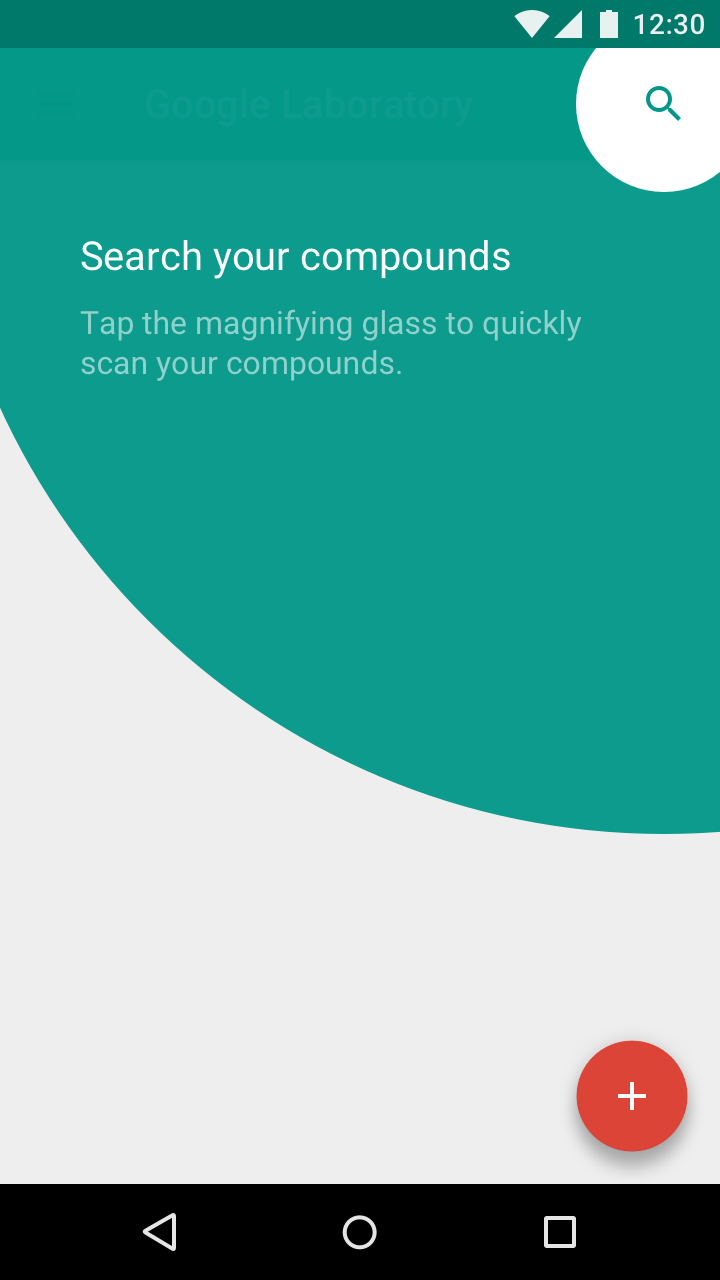
\includegraphics[keepaspectratio, width=0.5\textwidth]{fd}
% \caption{Feature-Discovery in Form eines Tap-Targets}
% \label{fig:fd}
% \end{figure}

% In \autoref{fig:fd} sieht man eine beispielhafte Implementierung einer solchen Feature-Discovery in Form eines Tap-Targets.
% Hierbei wird der Benutzer durch eine Hervorhebung bestimmter UI-Elemente auf Funktionen hingewiesen. 
% Zusätzlich wird ein kurzer erklärender Satz mit einem zusammenfassenden Titel angezeigt. \\

% \subsection{Gesture-Support}

% Mit der Einführung Applikationen für mobile Endgeräte hat sich ein weiteres, vorher nicht relevantes, Usability-Problem etabliert: 
% \emph{Die geringe Größe des Bildschirm}. \\

% Die relativ kleine physikalische Größe der Smartphone-Displays bringt verschiedene Probleme mit sich. 
% So muss einerseits die Funktionalität einer ganzen Desktop-Applikation auf ein viel kleineres Display passen, ohne den Content zu verändern, oder gar unleserlich zu machen.
% Andererseits muss dem Benutzer eine intuitive und effiziente Navigationsmöglichkeit gegeben sein, um zwischen verschiedenen Inhalten zu wechseln. \\

% Hierzu schreiben \citeauthor{Gutwin04}, dass die Navigationen auf kleinen Bildschirmen selbst im besten Fall deutlich langsamer sei als auf normal-großen Bildschirmen.
% Sie führen weiter an, dass eine Übersicht über den gesamten Systemzustand wertvoll sei, da dies dem Nutzer eine schnellere Navigation erlaube. \\
% Nach \citeauthor{Gutwin04} eigne sich die Technik des ``Two-Level Zooms'' besonders gut für Navigationsaufgaben, wohingegen Panning-Strategien eher negativ von den Test-Personen aufgenommen worden seien \citep[Seite 8]{Gutwin04}.  
